% \iffalse meta-comment
%
% Copyright (C) 2015 by Michael Muehlberghuber, IIS, ETH Zurich
%
% This program is free software: you can redistribute it and/or modify
% it under the terms of the GNU General Public License as published by
% the Free Software Foundation, either version 3 of the License, or
% (at your option) any later version.
% 
% This program is distributed in the hope that it will be useful,
% but WITHOUT ANY WARRANTY; without even the implied warranty of
% MERCHANTABILITY or FITNESS FOR A PARTICULAR PURPOSE.  See the
% GNU General Public License for more details.
% 
% You should have received a copy of the GNU General Public License
% along with this program.  If not, see <http://www.gnu.org/licenses/>.
%
% \fi
%
% \iffalse
%<*driver>
\ProvidesFile{iisbeamer.dtx}[2015/09/10 v0.1 IIS beamer theme]
%</driver>
%
%<*driver>
\documentclass[a4paper,11pt]{ltxdoc}
\usepackage{xspace}
\usepackage[textsize=scriptsize,colorinlistoftodos]{todonotes}
\usepackage{hyperref}
\EnableCrossrefs
\CodelineIndex
\RecordChanges
\begin{document}
 \DocInput{beamerthemeiis.dtx}
 \PrintChanges
 \PrintIndex
\end{document}
%</driver>
% \fi
%
% \CheckSum{0}
%
% \CharacterTable
%  {Upper-case    \A\B\C\D\E\F\G\H\I\J\K\L\M\N\O\P\Q\R\S\T\U\V\W\X\Y\Z
%   Lower-case    \a\b\c\d\e\f\g\h\i\j\k\l\m\n\o\p\q\r\s\t\u\v\w\x\y\z
%   Digits        \0\1\2\3\4\5\6\7\8\9
%   Exclamation   \!     Double quote  \"     Hash (number) \#
%   Dollar        \$     Percent       \%     Ampersand     \&
%   Acute accent  \'     Left paren    \(     Right paren   \)
%   Asterisk      \*     Plus          \+     Comma         \,
%   Minus         \-     Point         \.     Solidus       \/
%   Colon         \:     Semicolon     \;     Less than     \<
%   Equals        \=     Greater than  \>     Question mark \?
%   Commercial at \@     Left bracket  \[     Backslash     \\
%   Right bracket \]     Circumflex    \^     Underscore    \_
%   Grave accent  \`     Left brace    \{     Vertical bar  \|
%   Right brace   \}     Tilde         \~}
%
% \changes{v0.1}{2015/09/10}{Initial version}
%
% \GetFileInfo{beamerthemeiis.dtx}
%
% \DoNotIndex{\#,\$,\%,\@,\\,\{,\},\^,\_,\~,\ ,\"}
% \DoNotIndex{\let,\def,\else,\empty,\ensuremath,\iflanguage,\ifthenelse,\ifx,\isempty}
% \DoNotIndex{\textbf,\textsc,\textwidth,\vspace,\xspace,\url,\whiledo}
% \DoNotIndex{\value,\vfill,\newcommand,\fi,\global,\end}
% \DoNotIndex{\AtBeginDocument,\baselineskip,\begin,\CurrentOption,\DeclareOption}
% \DoNotIndex{\fontfamily,\fontseries,\fontsize,\hookleftarrow,\hrulefill,\Huge}
% \DoNotIndex{\itshape,\LARGE,\linewidth,\mbox,\newcounter,\newenvironment,\relax}
% \DoNotIndex{\@waferpngfalse,\@waferpngtrue,\if@waferpng,\mode,\newif,\ProcessOptions}
% \DoNotIndex{\RequirePackage,\setlength,\TPHorizModule,\TPVertModule}
% \DoNotIndex{\usecolortheme,\usefonttheme,\useinnertheme,\useoutertheme}
% \DoNotIndex{\definecolor,\setbeamercolor}
%
% \newcommand{\latexcls}[1]{\textsf{#1}}
% \newcommand{\latexsty}[1]{\textsf{#1}}
% \newcommand{\package}[1]{\textsf{#1}}
% \newcommand{\theme}[1]{\textsf{#1}}
% \newcommand{\file}[1]{\texttt{#1}}
% \newcommand{\option}[1]{\textsf{#1}}
% \newcommand{\name}[1]{#1}
% \newcommand{\mail}[1]{\texttt{#1}}
% \newcommand{\todoin}[1]{\todo[inline,size=\normalsize]{#1}\xspace}
% \newcommand{\texlive}{\TeX{}Live\xspace}
%
% \title{The \theme{iis} \latexcls{beamer} theme\thanks{This
%   document corresponds to \theme{iis}~\fileversion, dated~\filedate.}}
% \author{\name{Michael Muehlberghuber} \\ \mail{mbgh@iis.ee.ethz.ch}}
%
% \maketitle
%
% \begin{abstract}
%   The \theme{iis} theme for the \LaTeX{} \latexcls{beamer} class has
%   been developed at the Integrated Systems Laboratory (IIS). The
%   main purpose of the theme is to provide a minimalist layout with
%   regard to the space occupied by \emph{surrounding elements} such
%   as navigation bars, footer, or header and should basically work
%   out of the box at any workstation of the IIS IT
%   infrastructure. Thereby, most of the slide space can be filled
%   with actual content of the respective presentation.
% \end{abstract}
%
% \listoftodos
% \tableofcontents
%
% \section{Introduction}
% \todoin{Insert a small intro.}
%
% \section{Usage}
% \todoin{Describe the usage of the theme.}
%
% \section{Options}
% \todoin{Describe the available theme options.}
%
% \section{Commands}
% \todoin{Describe the provided commads.}
%
% \section{Caveats}
%
% \begin{itemize}
% \item The \theme{iis} \latexcls{beamer} theme has been designed to
%   work out of the box on the workstations of the Integrated Systems
%   Laboratory (IIS) using at least \texlive version
%   2011. Nevertheless, only minor adaptions should be necessary
%   (e.g., installing additional packages) to use it on any other
%   mature \TeX{} distribution.
% \end{itemize}
%
%
% \section{Known Bugs}
% \todoin{List the known bugs.}
%
% \section{Requested and Upcoming Features}
% \todoin{List the requested and upcoming features.}
%
% ^^A Indicate the start of the implementation part. This is important
% ^^A since the \CheckSum{} macro only counts the backslashes of the
% ^^A code (i.e., the lines not starting with a %) betwen the
% ^^A \StopEventually{} and the \Finale macro.
% \StopEventually{}
%
% \section{Implementation}
% Describe the structure of the theme here...
%
%
%
% \subsection{Main Theme File (\file{beamerthemeiis.sty})}
%
% \iffalse
%<*beamerthemeiis>
% \fi
%
% Ensure that the following changes are valid for all
% \emph{presentation} modes of \latexcls{beamer} (i.e., not for the
% \emph{article} mode).
%    \begin{macrocode}
\mode<presentation>
%    \end{macrocode}
%
% In the following, all the required packages are loaded. But first,
% let us summarize, why we actually need them:
% \begin{description}
%  \item[\latexsty{textpos}] For positioning the wafer image on the title page.
%  \item[\latexsty{tikz}] \todoin{TBD}
% \end{description}
%    \begin{macrocode}
\RequirePackage[absolute,overlay]{textpos}
\RequirePackage{tikz}
%    \end{macrocode}
%
% Setup the horizontal an vertical units for the \latexsty{textpos}
% package.
%    \begin{macrocode}
\setlength{\TPHorizModule}{1cm}
\setlength{\TPVertModule}{1cm}
%    \end{macrocode}
%
% Declare a boolean, which determines whether we should use the PNG
% version of the wafer (or the JPG version) on the title page.
%    \begin{macrocode}
\newif\if@waferpng
\@waferpngfalse
%    \end{macrocode}
%
% Declare the provided class options and process them.
%    \begin{macrocode}
\DeclareOption{waferpng}{\@waferpngtrue}
\ProcessOptions
%    \end{macrocode}
%
% Declare the settings (i.e., colors, fonts, as well as the inner and
% outer styles) for the \theme{iis} theme.
%    \begin{macrocode}
\usecolortheme{iis}
\usefonttheme{iis}
\useinnertheme{iis}
\useoutertheme{iis}
%    \end{macrocode}
%
% Ensure that all subsequent commands will again be valid for all
% modes of the \latexcls{beamer} class.
%    \begin{macrocode}
\mode<all>
%    \end{macrocode}
% \iffalse
%</beamerthemeiis>
% \fi
%
%
% \subsection{Outer Theme Settings (\file{beamerouterthemeiis.sty})}
%
% \iffalse
%<*beamerouterthemeiis>
% \fi
%
% Ensure that the following changes are valid for all
% \emph{presentation} modes of \latexcls{beamer} (i.e., not for the
% \emph{article} mode).
%    \begin{macrocode}
\mode<presentation>
%    \end{macrocode}
%
% Declare the frame title.
%    \begin{macrocode}
\defbeamertemplate*{frametitle}{iis}[1][left]
{%
\ifbeamercolorempty[bg]{frametitle}{}{\nointerlineskip}%
  \@tempdima=\textwidth%
  \advance\@tempdima by\beamer@leftmargin%
  \advance\@tempdima by\beamer@rightmargin%
  \begin{beamercolorbox}[%
    sep=0.0cm,leftskip=1.3em,wd=\the\@tempdima]{frametitle}
    \usebeamerfont{frametitle}%
    \vbox{}\vskip0.5ex%
    \if@tempswa\else\csname beamer@fteleft\endcsname\fi%
    {\strut\insertframetitle\strut\par%
    {%
      \ifx\insertframesubtitle\@empty%
      \else%
      {\usebeamerfont{framesubtitle}%
        \usebeamercolor[fg]{framesubtitle}%
        \insertframesubtitle\strut\par}%
      \fi
    }%
    \vskip-1.5ex%
    \rule{\dimexpr\paperwidth-0.6cm-1.5em\relax}{0.4pt}}
    \if@tempswa\else\vskip-.3cm\fi%
  \end{beamercolorbox}%
}
%    \end{macrocode}
%
% Create the frame header line.
%    \begin{macrocode}
\defbeamertemplate*{headline}{iis}
{%
  \leavevmode%
  \hbox{%
  \begin{beamercolorbox}[%
    wd=\paperwidth,ht=2.5ex,dp=1ex]{section in head/foot}%
    \usebeamerfont{section in head/foot}%
    \insertsectionnavigationhorizontal{\paperwidth}{}{}
  \end{beamercolorbox}}%
  \vskip0pt%
}
%    \end{macrocode}
%
% Create the frame footer line.
%    \begin{macrocode}
\defbeamertemplate*{footline}{iis}
{%
  \leavevmode%
  \hbox{%
  \begin{beamercolorbox}[%
    wd=\paperwidth,ht=2.5ex,dp=1ex]{palette tertiary}%
    \begin{beamercolorbox}[%
      wd=0.15\paperwidth,leftskip=0.32cm]{image in head/foot}%
      
\includegraphics[height=1.55ex]{eth_logo_neg}
    \end{beamercolorbox}%
    \begin{beamercolorbox}[%
      wd=0.7\paperwidth,center]{institute in head/foot}%
      \usebeamerfont{institute in head/foot}%
      \usebeamercolor[fg]{institute in head/foot}%
      \insertshortauthor\expandafter\beamer@ifempty%
      \expandafter{\beamer@shortinstitute}{}{~(\insertshortinstitute)}
    \end{beamercolorbox}%
    \begin{beamercolorbox}[%
      wd=0.15\paperwidth,right,rightskip=0.3cm]{%
        frame numbers in head/foot}%
      \usebeamerfont{frame numbers in head/foot}%
      \usebeamercolor[fg]{frame numbers in head/foot}%
      \insertframenumber{} / \inserttotalframenumber
    \end{beamercolorbox}%
  \end{beamercolorbox}}%
  \vskip0pt%
}
%    \end{macrocode}
%
% Ensure that we have a little bit less margin on the left and right
% of the actual content of the slides.
%    \begin{macrocode}
\setbeamersize{text margin left=2em,text margin right=2em}
%
%    \end{macrocode}
% Ensure that all subsequent commands will again be valid for all
% modes of the \latexcls{beamer} class.
%    \begin{macrocode}
\mode<all>
%    \end{macrocode}
%
% \iffalse
%</beamerouterthemeiis>
% \fi
%
%
% \subsection{Inner Theme Settings (\file{beamerinnerthemeiis.sty})}
%
% \iffalse
%<*beamerinnerthemeiis>
% \fi
%
% Ensure that the following changes are valid for all
% \emph{presentation} modes of \latexcls{beamer} (i.e., not for the
% \emph{article} mode).
%    \begin{macrocode}
\mode<presentation>
%    \end{macrocode}
%
% Per default, use the \emph{rectangles} inner theme in order to use,
% for instance, squares in the table of contents and in item
% environments.
%    \begin{macrocode}
\useinnertheme{rectangles}
%    \end{macrocode}
%
% Create some commands for positioning the wafer on the title page.
%    \begin{macrocode}
\def\@waferwidth{0.5}%
\newcommand{\setwaferwidth}[1]{\def\@waferwidth{#1}}%
\let\waferwidth\setwaferwidth%
%
\def\@waferleft{0.0}%
\newcommand{\setwaferleft}[1]{\def\@waferleft{#1}}%
\let\waferleft\setwaferleft%
%
\def\@wafertop{0.0}%
\newcommand{\setwafertop}[1]{\def\@wafertop{#1}}%
\let\wafertop\setwafertop%
%    \end{macrocode}
%
% Declare the title page.
%    \begin{macrocode}
\defbeamertemplate*{title page}{iis}[1][]
{ 
  \setbeamertemplate{headline}{}
  % Align all of the content on the title page to the right.
  \begin{flushright}
    % Insert the title.
    {\usebeamerfont{title}\usebeamercolor[fg]{title}%
      \textbf{\inserttitle}\vskip-0.2cm}%
    % Insert a horizontal rule.
    {\textcolor{structure.fg}{\rule{\linewidth}{2pt}}}%
    % Insert the subtitle (if specified by the user).
    \ifx\insertsubtitle\@empty\else%
    {\\\usebeamerfont{subtitle}\usebeamercolor[fg]%
      {title}\textbf{\insertsubtitle}}%
    \fi%
    {\\\usebeamerfont{date}{\footnotesize\insertdate}}%
    \vfill%
    {\usebeamerfont{author}{\small\insertauthor}}%
    \vfill%
    
\includegraphics[width=2cm]{eth_logo}\\%
    \usebeamerfont{institute}{\insertinstitute}%
  \end{flushright}
  % Place the wafer image (either the PNG version or the JPG version,
  % depending on the theme options specified).
  \begin{textblock}{12.8}(\@waferleft,\@wafertop)%
    \if@waferpng%
    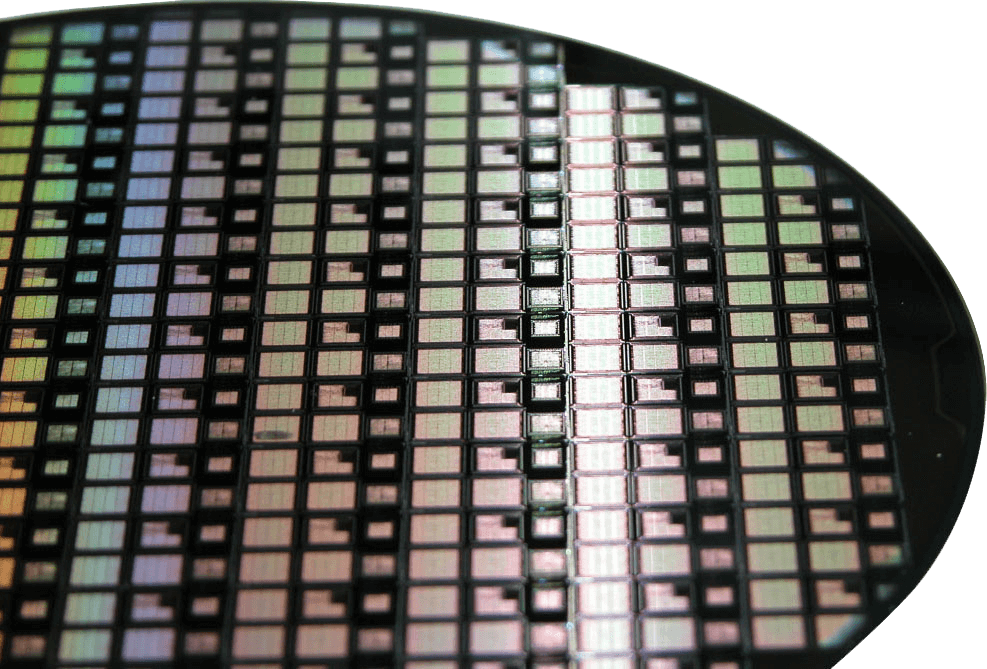
\includegraphics[width=\@waferwidth\linewidth]{wafer.png}%
    \else%
    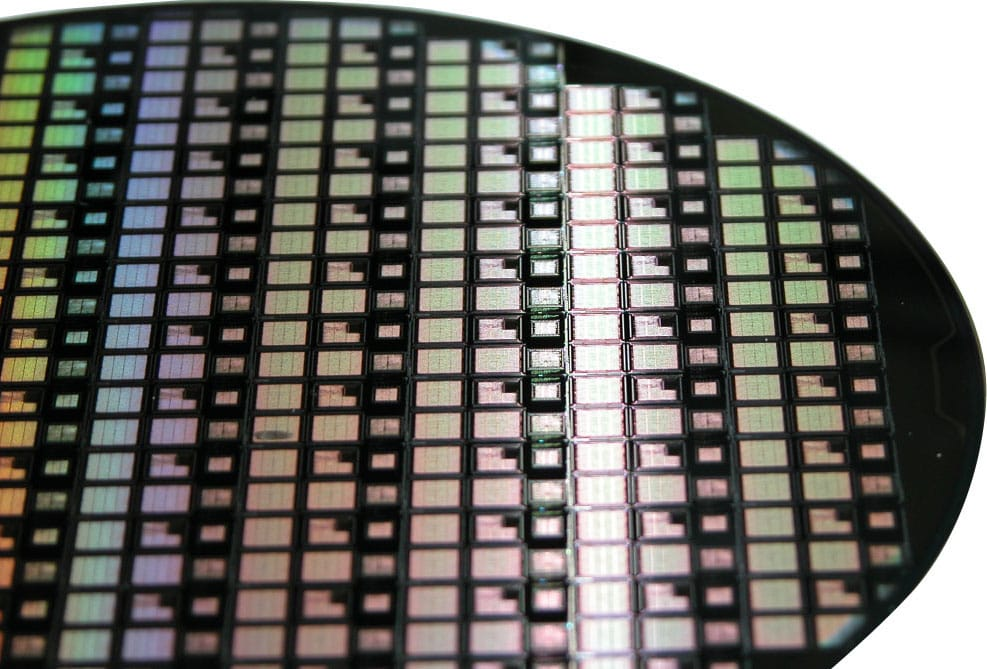
\includegraphics[width=\@waferwidth\linewidth]{wafer.jpg}%
    \fi%
  \end{textblock}%
}
%    \end{macrocode}
%
% Make sure the item environmens are left-aligned with the actual text
% of a slide.
%    \begin{macrocode}
\setlength{\leftmargini}{1em}
\setlength{\leftmarginii}{1.2em}
%    \end{macrocode}
%
% Make sure that all block environments have rounded edges.
%    \begin{macrocode}
\setbeamertemplate{blocks}[rounded]
%    \end{macrocode}
% TBD:
%    \begin{macrocode}
\defbeamertemplate{description item}{align left}%
{\insertdescriptionitem\hfill}
%    \end{macrocode}
%
% Ensure that all subsequent commands will again be valid for all
% modes of the \latexcls{beamer} class.
%    \begin{macrocode}
\mode<all>
%    \end{macrocode}
%
% \iffalse
%</beamerinnerthemeiis>
% \fi
%
%
% \subsection{Color Settings (\file{beamercolorthemeiis.sty})}
%
% \iffalse
%<*beamercolorthemeiis>
% \fi
%
% Ensure that the following changes are valid for all
% \emph{presentation} modes of \latexcls{beamer} (i.e., not for the
% \emph{article} mode).
%    \begin{macrocode}
\mode<presentation>
%    \end{macrocode}
%
% Declare the ETH corporate design
% colors\footnote{\url{https://www.ethz.ch/services/en/service/communication/corporate-design/colour.html}} based on RGB values.
%    \begin{macrocode}
\definecolor{eth1}{RGB}{31,64,122}
\definecolor{eth2}{RGB}{72,90,44}
\definecolor{eth3}{RGB}{18,105,176}
\definecolor{eth4}{RGB}{114,121,28}
\definecolor{eth5}{RGB}{145,5,105}
\definecolor{eth6}{RGB}{111,111,100}
\definecolor{eth7}{RGB}{168,50,45}
\definecolor{eth8}{RGB}{0,122,150}
\definecolor{eth9}{RGB}{149,96,19}
\definecolor{eth10}{RGB}{140,182,60}
%    \end{macrocode}
%
% Declare the main color of the theme.
%    \begin{macrocode}
\setbeamercolor*{structure}{fg=eth1}
%    \end{macrocode}
%
% Derive the color palettes for the outer theme from the main color.
%    \begin{macrocode}
\setbeamercolor{palette primary}{%
  use=structure,fg=white,bg=structure.fg!40!white}
\setbeamercolor{palette secondary}{%
  use=structure,fg=white,bg=structure.fg!60!white}
%    \end{macrocode}
%
% Note that the following color is used for the headers and footers.
%    \begin{macrocode}
\setbeamercolor{palette tertiary}{%
  use=structure,fg=white,bg=structure.fg!90!white}
\setbeamercolor{palette quaternary}{%
  fg=white,bg=black}
%    \end{macrocode}
%
% Specify the colors of the standard block.
%    \begin{macrocode}
\setbeamercolor{block title}{%
  parent=normal text,fg=white,bg=eth1}
\setbeamercolor{block body}{%
  parent=normal text,use=block title,bg=block title.bg!20!bg}
%    \end{macrocode}
%
% Specify the colors of the example block.
%    \begin{macrocode}
\setbeamercolor{example text}{fg=eth4}
\setbeamercolor{block title example}{%
  use=example text,fg=white,bg=example text.fg}
\setbeamercolor{block body example}{%
  parent=normal text,use=block title example,%
  bg=block title example.bg!20!bg}
%    \end{macrocode}
%
% Specify the colors of the alert box.
%    \begin{macrocode}
\setbeamercolor{alerted text}{fg=eth7}
\setbeamercolor{alerted block}{fg=eth7}
\setbeamercolor{block title alerted}{%
  use=alerted block,fg=white,bg=alerted block.fg}
\setbeamercolor{block body alerted}{%
  parent=normal text,use=block title alerted,%
  bg=block title alerted.bg!20!bg}
%    \end{macrocode}
%
% Ensure that all subsequent commands will again be valid for all
% modes of the \latexcls{beamer} class.
%    \begin{macrocode}
\mode<all>
%    \end{macrocode}
%
% \iffalse
%</beamercolorthemeiis>
% \fi
%
%
% \subsection{Font Settings (\file{beamercolorthemeiis.sty})}
%
% \iffalse
%<*beamerfontthemeiis>
% \fi
%
% Ensure that the following changes are valid for all
% \emph{presentation} modes of \latexcls{beamer} (i.e., not for the
% \emph{article} mode).
%    \begin{macrocode}
\mode<presentation>
%    \end{macrocode}
%
% Set the font for the frame titles.
%    \begin{macrocode}
\setbeamerfont{frametitle}{series=\bfseries}
%    \end{macrocode}
%
% Ensure that all subsequent commands will again be valid for all
% modes of the \latexcls{beamer} class.
%    \begin{macrocode}
\mode<all>
%    \end{macrocode}
%
% \iffalse
%</beamerfontthemeiis>
% \fi
%
% \Finale
%
\endinput
